% ============================================================
%  Semiring-Based Multimodal Routing  Final Project Report
%  References: CLRS §24 · ACT4E §14.1/14.3/14.6
% ============================================================
\documentclass[12pt,a4paper]{article}

% ---------- Packages ----------
\usepackage[T1]{fontenc}
\usepackage[utf8]{inputenc}
\usepackage{geometry}
\geometry{margin=2.5cm}

\usepackage{mdframed}
\usepackage{amsmath,amssymb,amsthm}
\usepackage{mathtools}
\usepackage{booktabs}
\usepackage{array}
\usepackage{tabularx}
\usepackage{multirow}
\usepackage{graphicx}
\usepackage{float}
\usepackage{caption}
\usepackage{subcaption}
\usepackage{hyperref}
\hypersetup{hidelinks,pdfborder={0 0 0}}
\usepackage{xcolor}
\usepackage{listings}
\usepackage{algorithm}
\usepackage{algpseudocode}
\usepackage{enumitem}
\usepackage{setspace}
\usepackage{fancyhdr}
\usepackage{tikz}
\usetikzlibrary{arrows.meta,positioning,shapes.geometric}

\onehalfspacing

% ---------- Theorem environments ----------
\newtheorem{definition}{Definition}[section]
\newtheorem{theorem}{Theorem}[section]
\newtheorem{lemma}{Lemma}[section]
\newtheorem{proposition}{Proposition}[section]
\newtheorem{remark}{Remark}[section]
\newtheorem{example}{Example}[section]

% ---------- Code style ----------
\definecolor{codegray}{rgb}{0.95,0.95,0.95}
\lstset{
  backgroundcolor=\color{codegray},
  basicstyle=\ttfamily\small,
  breaklines=true,
  frame=single,
  columns=fullflexible,
  keepspaces=true,
  showstringspaces=false
}

% ---------- Macros ----------
\newcommand{\SR}{\mathbb{S}}
\newcommand{\Rzero}{\bar{0}}
\newcommand{\Rone}{\bar{1}}
\newcommand{\opl}{\oplus}
\newcommand{\otm}{\otimes}
\newcommand{\R}{\mathbb{R}}
\newcommand{\Z}{\mathbb{Z}}
\newcommand{\N}{\mathbb{N}}
\newcommand{\Trop}{(\R,\min,+,\infty,0)}
\newcommand{\BN}{(\R,\max,\min,-\infty,+\infty)}

% ---------- Header / Footer ----------
\pagestyle{fancy}
\fancyhf{}
\lhead{\small Semiring-Based Multimodal Routing}
\rhead{\small \thepage}
\renewcommand{\headrulewidth}{0.4pt}

\title{\textbf{Semiring-Based Dijkstra for Multimodal Route Planning}\\
\large Course Project Report for SL203: Introduction to Algorithms and Software Programming}
\author{Kartikeya Gaur (26371)\\CiSTUP, Indian Institute of Science, Bengaluru}
\date{April 2026}

\begin{document}

\begin{titlepage}

\vspace{-2cm}

\centering

{\LARGE \bfseries Semiring-Based Dijkstra for Multimodal Route Planning}

\vspace{1\baselineskip}


{\LARGE \bfseries Course Project Report}

\vspace{1\baselineskip}


{\Large \bfseries SL203: Introduction to Algorithms and Software Programming

\vspace{0.5\baselineskip}


{\Large in}

\vspace{0.5\baselineskip}


{\Large \bfseries M.Tech Programme }

\vspace{0.5\baselineskip}


{\Large by}


{\Large \bfseries Kartikeya Gaur (26371)}

\vspace{1\baselineskip}


{\Large Supervisor: \bfseries Dr. Nagarajan Natarajan}

\vspace{1\baselineskip}


\includegraphics[width=0.3\linewidth]{logo.png}

\vspace{1\baselineskip}


{\Large CiSTUP}

%\vspace{0.5\baselineskip}


{\Large Indian Institute of Science, Bangalore}

%\vspace{.5\baselineskip}


{\Large Bangalore-560012}

\vspace{.5\baselineskip}



{\Large \textbf{May, 2026}}}


\end{titlepage}

\begin{abstract}
    \noindent
    This report presents a generalised routing engine for the inner Bengaluru
    multimodal network (road + BMTC bus) whose design separates graph topology
    from cost algebra.  The same Dijkstra backbone operates on a single
    intermodal graph $G = G_r \cup G_b \cup G_t$, while interchangeable
    \emph{semiring} instances encode distance, travel time, fare, safety, or
    lexicographic combinations thereof.  The mathematical basis draws from two
    complementary traditions: the \emph{tropical-semiring} and
    \emph{semiring-shortest-distance} framework of Mohri~\cite{mohri2002}, the
    \emph{dioid} perspective on algebraic path problems of Gondran and
    Minoux~\cite{gondran2008}, and the categorical treatment of routing
    networks in Fong and Spivak's \emph{Applied Category Theory}
    \cite{fong2019} and the \emph{ACT4E} notes~\cite{act4e}.  The algorithmic
    analysis follows the CLRS treatment of single-source shortest-path
    algorithms~\cite{clrs}.  A working Python prototype demonstrates that
    fixed-objective semiring routing is often more practical than full
    Pareto-front enumeration within a unified multimodal state-space.
\end{abstract}
\newpage
\tableofcontents
\newpage

% ============================================================
\section{Introduction}
\label{sec:intro}

\subsection{Problem Statement}

The motivation for transitioning toward enriched categories in multimodal routing stems from the inherent limitations of traditional graph-based optimization. While Pareto-optimal sets are mathematically sound, they are effectively "useless at scale" because they grow exponentially as more criteria are added. Even advanced algorithmic frameworks like McRAPTOR and BM-RAPTOR struggle to overcome this; they face a significant technical bottleneck where parallelization provides a meager 1.7 times speedup. Some state-of-art algorithams delivers the near-instantaneous (roughly 30ms) response times required for real-world applications but only for 2-3 criterias, what if we are to expand. Refer Figure~\ref{fig:problems}.

\begin{figure}[H]
  \centering
  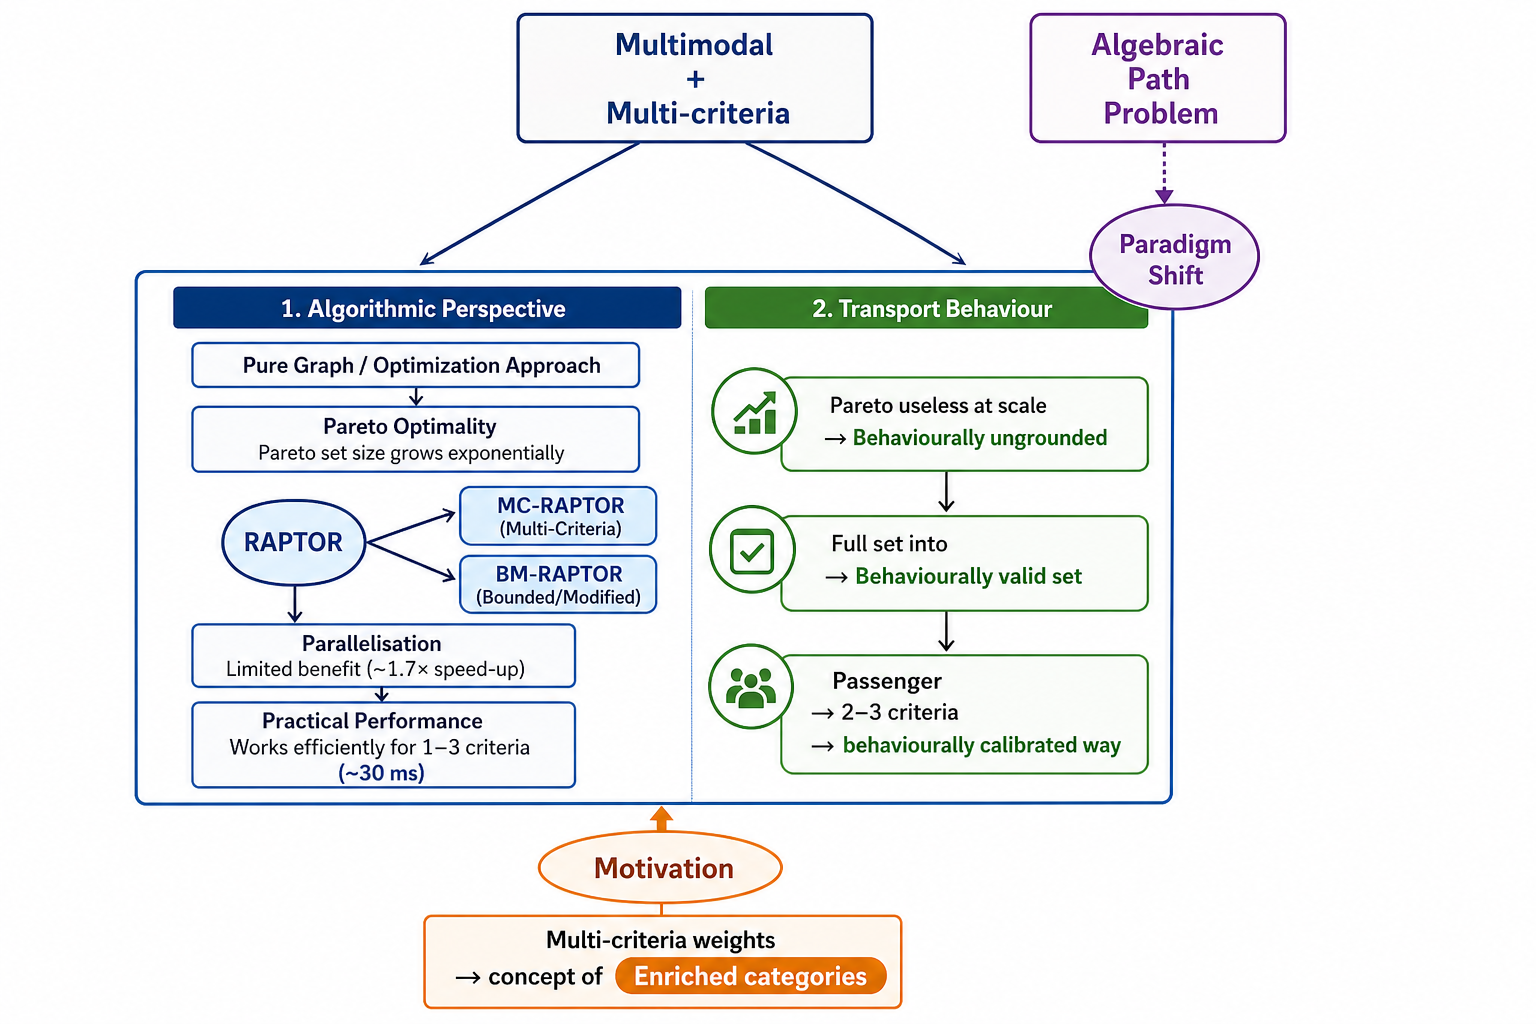
\includegraphics[width=0.85\textwidth]{overview.png}
  \caption{Multimodal routing overview.}
  \label{fig:problems}
\end{figure}

\begin{itemize}
  \item Lozano \& Storchi (2001) show that standard Dijkstra requires an
        \textbf{ad hoc} modification to handle multimodal networks.
  \item Zhang et al.\ (2013) establish that the general multi-criteria
        multi-modal shortest path problem is \textbf{NP-hard}.
  \item Potthoff \& Sauer (2021) note that efficient algorithms either
        \textbf{restrict} transfer usage or limit optimisation to
        \textbf{two criteria}.
\end{itemize}

The explosion of Pareto frontiers under multiple criteria isn't just a computational problem it's a sign that the algebraic structure being used (real-valued scalar costs) is the wrong enriching category. A richer algebraic structure (a tropical semiring, a lattice-ordered monoid, or a preordered commutative monoid) might represent multi-criteria costs in a way that admits efficient computation of "optimal" paths without full Pareto enumeration.

While adequate for single-mode distance minimisation, this rigidity becomes a
liability in \emph{multimodal} networks where cost semantics differ
radically across objectives:

\begin{itemize}[noitemsep]
  \item \textbf{Distance:} total metres travelled.
  \item \textbf{Time:} mode-dependent travel time plus waiting penalties.
  \item \textbf{Fare:} monetary cost in Rupees, with per-kilometre road and
        bus tariffs.
  \item \textbf{Safety:} bottleneck score  the weakest link along a path.
  \item \textbf{Lexicographic objectives:} time with fare as tie-breaker.
\end{itemize}

Each objective has a different algebra.  A bottleneck safety score requires
$\max \circ \min$ rather than $\min \circ +$.  A lexicographic objective
requires tuple comparison, not scalar addition.  Rebuilding five separate
routing engines would be both wasteful and error-prone.

\subsection{The Multimodal Challenge}

Multimodal networks introduce an additional layer of complexity: the
state space is no longer a set of physical locations $L$ but the Cartesian
product $V = L \times M$, where $M$ denotes the set of transport modes.
Edges must distinguish between:
\begin{itemize}[noitemsep]
  \item \textbf{Intramodal edges}  movement within a single mode (e.g.\ driving
        along a road segment).
  \item \textbf{Intermodal transfer edges}  mode switches at co-located nodes
        (e.g.\ walking from a road intersection to a nearby bus stop).
\end{itemize}
Transfer edges carry their own cost semantics: walking time, possible
boarding delays, and zero monetary fare but non-trivial safety scores.
The interaction between transfer costs and objective-specific algebras
makes naive Pareto-front computation computationally intractable for
real-time applications.

\subsection{Contribution}

This project delivers:
\begin{enumerate}[noitemsep]
  \item A \textbf{generalised solver} for the Algebraic Path Problem (APP)
        in Python, parameterised by an abstract \texttt{Semiring} interface.
  \item A \textbf{multimodal graph} for inner Bengaluru combining
        OpenStreetMap road data and BMTC bus routes, with explicit transfer
        edges.
  \item Six concrete semiring instances covering the objectives listed above.
  \item Empirical evaluation on five origin–destination pairs representative
        of key Bengaluru corridors.
  \item A categorical interpretation of the routing problem drawing on
        ACT4E §14.1 (mobility categories), §14.3 (enriched morphisms as
        cost-bearing arrows), and §14.6 (procedures with resource
        consumption).
\end{enumerate}

\begin{mdframed}[linewidth=1.2pt, linecolor=black,
                 backgroundcolor=gray!8,
                 innertopmargin=10pt, innerbottommargin=10pt,
                 innerleftmargin=14pt, innerrightmargin=14pt]
  \centering
  \textit{Same graph, same algorithmic skeleton, different algebra
  $\;\Longrightarrow\;$ different routing objective.}
\end{mdframed}
\vspace{0.5em}

% ============================================================
\section{Mathematical Foundations: Semirings}
\label{sec:semirings}

\subsection{Definition and Axioms}

\begin{definition}[Semiring]
  A \emph{semiring} is a quintuple $(\SR, \opl, \otm, \Rzero, \Rone)$
  satisfying:
  \begin{enumerate}
    \item $(\SR, \opl, \Rzero)$ is a commutative monoid:
          $a \opl b = b \opl a$,\; $(a \opl b) \opl c = a \opl (b \opl c)$,\;
          $a \opl \Rzero = a$.
    \item $(\SR, \otm, \Rone)$ is a monoid:
          $(a \otm b) \otm c = a \otm (b \otm c)$,\;
          $a \otm \Rone = \Rone \otm a = a$.
    \item $\otm$ distributes over $\opl$:
          $a \otm (b \opl c) = (a \otm b) \opl (a \otm c)$,\;
          $(b \opl c) \otm a = (b \otm a) \opl (c \otm a)$.
    \item $\Rzero$ is absorbing: $a \otm \Rzero = \Rzero \otm a = \Rzero$.
  \end{enumerate}
  The operator $\opl$ is called the \emph{choice} (or \emph{selection})
  operator; $\otm$ is the \emph{extension} (or \emph{path-cost}) operator.
\end{definition}

The interpretation in routing is immediate: $a \otm b$ extends a partial
path with cost $a$ by an edge of cost $b$, while $a \opl b$ selects the
preferred among two candidate costs at the same node.  The absorbing element
$\Rzero$ represents an ``unreachable'' state; $\Rone$ is the cost of the
trivial (empty) path at the source.

\subsection{Idempotency and the Induced Partial Order}

A semiring is \emph{idempotent} (or a \emph{dioid}~\cite{gondran2008}) if
\[
  a \opl a = a \quad \forall\, a \in \SR.
\]
Idempotency induces a canonical partial order:
\[
  a \leq b \iff a \opl b = a.
\]
Under this order, $a \leq b$ means ``$a$ is at least as good as $b$'' (i.e.\
$a$ is preferred).  This is precisely the condition needed for Dijkstra's
greedy selection step to remain correct: once a node is settled at cost $a$,
no future relaxation can produce a cost $a'$ with $a' \opl a \neq a$.

\begin{theorem}[Dijkstra Correctness for Idempotent Semirings]
  Let $(\SR, \opl, \otm, \Rzero, \Rone)$ be an idempotent semiring whose
  extension operator $\otm$ is \emph{monotone}: for all $a, b, c \in \SR$,
  $a \leq b \Rightarrow a \otm c \leq b \otm c$ and
  $c \otm a \leq c \otm b$.  Then the generalised Dijkstra algorithm
  (Algorithm~\ref{alg:gen-dijkstra}) terminates and computes correct
  $(\opl, \otm)$-shortest paths from the source.
\end{theorem}

Monotonicity ensures that extending a suboptimal path never produces an
optimal one  the analogue of the non-negative-weight assumption in the
classical setting (CLRS Theorem~24.6~\cite{clrs}).

\subsection{Semiring Instances}
\label{subsec:semiring-instances}

Table~\ref{tab:semiring-instances} summarises the semiring instances
relevant to this project, together with their identity elements and
suitability for Dijkstra.

\begin{table}[H]
\centering
\caption{Semiring instances and their routing semantics}
\label{tab:semiring-instances}
\renewcommand{\arraystretch}{1.3}
\begin{tabular}{l l c c l l}
\toprule
\textbf{Name} & $\mathbb{S}$ & $\oplus$ & $\otimes$ & $\bar{0}$ & $\bar{1}$ \\
\midrule
Tropical (distance / time / fare)
  & $\mathbb{R}_{\geq 0} \cup \{\infty\}$
  & $\min$ & $+$
  & $\infty$ & $0$ \\

Bottleneck (safety)
  & $[0,1]$
  & $\max$ & $\min$
  & $-\infty$ & $+\infty$ \\

Lexicographic
  & $\mathbb{R}^{2}$
  & $\mathrm{lex\text{-}min}$ & $+$
  & $(\infty,\infty)$ & $(0,0)$ \\

Transfer-penalised
  & $\mathbb{R}^{3}$
  & $\mathrm{score\text{-}min}$ & $+$
  & $(\infty,\infty,\infty)$ & $(0,0,0)$ \\

Integer (hop count)
  & $\mathbb{N} \cup \{\infty\}$
  & $\min$ & $+$
  & $\infty$ & $0$ \\
\bottomrule
\end{tabular}
\end{table}

\paragraph{Tropical semiring.}
The classical $(\R, +, \min, \infty, 0)$ semiring underlies distance, time,
and fare routing.  It is idempotent and monotone, so Dijkstra applies
directly (CLRS §24.3~\cite{clrs}).

\paragraph{Bottleneck (safety) semiring.}
For safety routing the \emph{bottleneck} or \emph{minimax} semiring
$(\R, \max, \min, -\infty, +\infty)$ is appropriate.  A path's cost is the
minimum safety score of its constituent edges; the algorithm maximises this
minimum.  Idempotency holds since $\max(a,a) = a$.  Monotonicity holds
because $\min(a, c) \leq \min(b, c)$ whenever $a \leq b$ under the $\max$
order.

\paragraph{Lexicographic semiring.}
Costs are pairs $(t, f) \in \R^2$.  The choice operator uses
lexicographic comparison: $(t_1, f_1) \opl (t_2, f_2)$ equals whichever
pair is lexicographically smaller.  The extension operator adds
component-wise.  This enforces strict time minimisation with fare as a
secondary criterion.

% ============================================================
\section{Categorical Modelling of Multimodal Networks}
\label{sec:category}

\subsection{Motivation: From Graphs to Categories}

The ACT4E framework~\cite{act4e} treats multimodal transport networks as
examples of \emph{categories enriched over a cost algebra}.  Section~14.1
of ACT4E introduces the \emph{mobility} use-case by composing separate
mode-specific graphs into an intermodal graph:

\begin{quote}
  ``By considering the graph $\mathcal{G} = (\mathbf{V}, \mathbf{E},
  \mathrm{src}, \mathrm{tgt})$ with $\mathbf{V} = \mathbf{V}^c \cup
  \mathbf{V}^s \cup \mathbf{V}^b$ and $\mathbf{E} = \mathbf{E}^c \cup
  \mathbf{E}^s \cup \mathbf{E}^b$, we obtain the desired intermodality
  graph \ldots\ which can be seen as a new category, with objects
  $\mathbf{V}$ and morphisms $\mathbf{E}$.'' \emph{(ACT4E §14.1)}
\end{quote}

Our Bengaluru graph is an instantiation of this construction with car
$\to$ road and subway $\to$ BMTC bus.

\subsection{Objects and Morphisms}

\begin{definition}[Multimodal State Space]
  Let $L$ denote the set of physical locations (OSM node identifiers) and
  $M = \{\texttt{road}, \texttt{bus}\}$ the set of transport modes.  The
  \emph{object set} of the routing category is
  \[
    V = L \times M.
  \]
  A state $(l, m) \in V$ represents being at location $l$ using mode $m$.
\end{definition}

Morphisms (edges) fall into three classes:
\begin{itemize}[noitemsep]
  \item \textbf{Intramodal:} $(l_1, m) \to (l_2, m)$ with $l_1 \neq l_2$
        and $m$ fixed  movement along a road segment or between consecutive
        bus stops.
  \item \textbf{Intermodal (transfer):} $(l, m_1) \to (l, m_2)$ with
        $m_1 \neq m_2$ and $l$ fixed  mode switch at a co-located
        road/bus node.
\end{itemize}
Composition of morphisms corresponds to path concatenation, which is
well-defined as long as the target of one morphism equals the source of the
next.  The identity morphism at $(l, m)$ is the zero-cost self-loop.

\subsection{Enrichment over a Semiring}

Following ACT4E §14.3 and §14.6, we enrich the routing category over the
semiring $(\SR, \opl, \otm, \Rzero, \Rone)$ by assigning to each morphism
$f \colon u \to v$ a \emph{weight} $w(f) \in \SR$.  The weight of a
composed path
\[
  u \xrightarrow{f_1} v_1 \xrightarrow{f_2} v_2 \cdots
  \xrightarrow{f_k} v
\]
is defined by iterated $\otm$:
\[
  w(f_k \circ \cdots \circ f_1) = w(f_1) \otm w(f_2) \otm \cdots \otm w(f_k).
\]
The ``best'' path from $u$ to $v$ is the one whose weight is optimal under
the partial order induced by $\opl$.  This is precisely the
\emph{Algebraic Path Problem} of Gondran and Minoux~\cite{gondran2008}.

ACT4E §14.6 (the \texttt{ProcTime} and \texttt{ProcSizeTime}
semicategories) provides a concrete precedent: morphisms carry execution
time as an additive annotation, composed by addition.  Our semiring
framework generalises this: instead of a single additive time annotation, a
morphism carries an element of an arbitrary semiring.

The connection between the categorical structure and the algorithmic one is
clean: Dijkstra's algorithm, interpreted categorically, computes for each
object $v$ the $(\opl, \otm)$-``best'' hom-set element from the source $s$
to $v$  that is, the optimal morphism $s \to v$ in the enriched category.

\subsection{State-ID Bijection}

To operate on standard adjacency lists in Python/C++, the categorical state
$(l, m)$ is mapped to a unique integer identifier via the bijection
\[
  f \colon L \times M \to \Z, \quad
  f(l, m) =
  \begin{cases}
    \mathrm{osm\_id}(l) & \text{if } m = \texttt{road},\\
    \mathrm{osm\_id}(l) + N & \text{if } m = \texttt{bus},
  \end{cases}
\]
where $N$ is an offset larger than the maximum OSM node identifier in the
subgraph.  This flattening is purely an implementation detail; the
categorical structure is preserved in the edge data (the \texttt{mode}
attribute on each edge records whether it is intramodal or intermodal).



% ============================================================
\section{Algorithmic Generalisation}
\label{sec:algorithms}

\subsection{Generalised Dijkstra}

Algorithm~\ref{alg:gen-dijkstra} presents Dijkstra's algorithm in abstract
semiring notation, replacing the hard-coded $\min$ and $+$ of
CLRS §24.3~\cite{clrs} with the abstract operators $\opl$ and $\otm$.

\begin{algorithm}[H]
\caption{Generalised Dijkstra over a semiring $(\SR, \opl, \otm, \Rzero, \Rone)$}
\label{alg:gen-dijkstra}
\begin{algorithmic}[1]
\Require Graph $G=(V,E)$, source $s \in V$, semiring $\mathcal{S}$
\Ensure $\mathrm{dist}[v]$: $(\opl, \otm)$-optimal cost from $s$ to $v$, $\forall v$
\State $\mathrm{dist}[v] \leftarrow \Rzero$ for all $v \in V$
\State $\mathrm{dist}[s] \leftarrow \Rone$
\State $Q \leftarrow V$ \Comment{priority queue keyed by $\mathrm{dist}$}
\While{$Q \neq \emptyset$}
  \State $u \leftarrow \arg\!\min_{\opl}\{{\rm dist}[v] : v \in Q,\; {\rm dist}[v] \neq \Rzero\}$
  \State remove $u$ from $Q$
  \For{each neighbour $v$ of $u$ with edge weight $w(u,v) \in \SR$}
    \State $\mathrm{relaxed} \leftarrow \mathrm{dist}[u] \otm w(u,v)$
    \If{$\mathrm{relaxed} \opl \mathrm{dist}[v] = \mathrm{relaxed}$}
      \Comment{$\mathrm{relaxed}$ is preferred over current $\mathrm{dist}[v]$}
      \State $\mathrm{dist}[v] \leftarrow \mathrm{relaxed}$
      \State $\mathrm{prev}[v] \leftarrow u$
    \EndIf
  \EndFor
\EndWhile
\end{algorithmic}
\end{algorithm}

The relaxation condition on line~9 is the semiring analogue of CLRS's
\texttt{RELAX} procedure.  When instantiated with the tropical semiring,
lines 9--10 reduce exactly to
$\mathrm{dist}[v] \leftarrow \min(\mathrm{dist}[v],\; \mathrm{dist}[u] + w(u,v))$,
recovering the classical algorithm.

\subsection{Convergence and Correctness}

The convergence argument mirrors CLRS Theorem~24.6.  Let $S$ denote the
set of vertices whose optimal costs have been finalised.  The loop invariant
is:
\begin{quote}
  At the start of each iteration, $\mathrm{dist}[v]$ equals the true
  $(\opl, \otm)$-optimal cost from $s$ to $v$, for all $v \in S$.
\end{quote}
Monotonicity of $\otm$ ensures that extracting the minimum-$\opl$ vertex
$u$ from $Q$ is safe: no future path through an unsettled vertex can produce
a cost preferred over $\mathrm{dist}[u]$.  The formal proof is a
straightforward generalisation of the CLRS proof by contradiction (CLRS
pp.~659--661).

\subsection{Bellman--Ford}

For the \emph{fare semiring} with negative weights (modelling government
subsidies injected as negative edge costs), Dijkstra is incorrect and
Bellman--Ford is required.  The CLRS §24.1 Bellman--Ford pseudocode
\cite{clrs} applies directly: perform $|V|-1$ rounds of full-graph edge
relaxation, then check for further improvements to detect negative-weight
cycles.  In our implementation a $\text{Rs}\,20$ fare subsidy on a selected
road segment is used to demonstrate this failure mode and validate that
Bellman--Ford produces the globally optimal subsidised fare path.

\subsection{Complexity}

\begin{itemize}[noitemsep]
  \item \textbf{Tropical Dijkstra (binary heap):} $O((V+E)\log V)$.
        Follows CLRS §24.3 directly.
  \item \textbf{Generic semiring Dijkstra ($O(V^2)$ select-best):}
        Used for non-totally-ordered carriers (safety, lexicographic,
        transfer semirings).  Complexity is $O(V^2 + E)$  acceptable for
        the Bengaluru subgraph ($\lvert V \rvert \lesssim 10^4$).
  \item \textbf{Bellman--Ford:} $O(V \cdot E)$  used only for
        negative-weight fare demonstration.
\end{itemize}
All complexity figures are invariant to the semiring carrier type, assuming
$O(1)$ for the $\opl$ and $\otm$ operators.

% ============================================================
\section{System Architecture \& Implementation}
\label{sec:architecture}

\subsection{Overview}

The system implements a multimodal routing engine for inner Bengaluru
that unifies road and BMTC bus networks into a single intermodal graph
$G = G_r \cup G_b \cup G_t$, then applies Dijkstra's algorithm
generalised over four distinct semiring weight algebras.
The architecture is divided into five modules
(\texttt{bus\_graph.py}, \texttt{graph\_setup.py},
\texttt{semirings.py}, \texttt{dijkstra.py},
\texttt{bellman\_ford.py}) and a top-level orchestration entry point
(\texttt{main.py}).

\begin{mdframed}[linewidth=1pt, linecolor=black, backgroundcolor=gray!8,
                 innertopmargin=8pt, innerbottommargin=8pt]
  \footnotesize\sloppy
  \textbf{Source code:}\quad
  All implementation described in this section is publicly available at
  \url{https://github.com/kartikeya-gaur/Semiring-based-Dijkstra}

  \smallskip
  The repository contains four versioned folders:
  \texttt{ch4\_v3} (road-only baseline),
  \texttt{claude\_v6\_git/ch4\_v3} (bus graph added),
  \texttt{cpp\_pareto\_semiring\_v7} (C\texttt{++} Pareto extension), and
  \texttt{final\_version\_v8} (final submission, 11 commits).
\end{mdframed}
\vspace{0.8em}

\subsection{Graph Construction}

\subsubsection{Road Sub-graph $G_r$}

The road network is downloaded from OpenStreetMap via the
\texttt{osmnx} library as a directed multigraph, centred on MG~Road
at latitude $12.9716°\,\mathrm{N}$, longitude
$77.5946°\,\mathrm{E}$, with a bounding radius of $5\,\mathrm{km}$.
Each road node is represented as a \texttt{(osm\_id,\;`road')} tuple.
Edge attributes retained include \texttt{highway}, \texttt{length} (metres),
and a derived \texttt{mode = `road'} tag.
Speed and safety values are resolved from the road-class lookup in
Table~\ref{tab:road-params}.

\begin{table}[H]
\centering
\caption{Road-class speed and safety parameters}
\label{tab:road-params}
\begin{tabular}{lrr}
\toprule
\textbf{Highway type} & \textbf{Speed (km/h)} & \textbf{Safety score} \\
\midrule
\texttt{motorway}       & 80 & 0.45 \\
\texttt{trunk}          & 65 & 0.55 \\
\texttt{primary}        & 50 & 0.65 \\
\texttt{secondary}      & 40 & 0.75 \\
\texttt{tertiary}       & 35 & 0.82 \\
\texttt{residential}    & 25 & 0.92 \\
\texttt{living\_street} & 15 & 0.95 \\
\texttt{unclassified}   & 30 & 0.80 \\
\bottomrule
\end{tabular}
\end{table}

\subsubsection{Bus Sub-graph $G_b$}

The bus network is fetched from the Overpass API, querying for OSM
relations tagged \texttt{route=bus} and \texttt{operator=BMTC} within a
bounding box covering inner Bengaluru.  A synthetic fallback dataset
activates automatically on API unavailability.  Bus-stop nodes are encoded
as \texttt{(osm\_id,\;`bus')} tuples.  Each directed edge between consecutive
stops carries \texttt{mode = `bus'}, a Haversine \texttt{length} (metres),
and BMTC route identifiers.  Assumed parameters: average bus speed
$18\,\mathrm{km/h}$, average waiting time $600\,\mathrm{s}$, fare
$1.5\,\mathrm{Rs/km}$.

\subsubsection{Transfer Edges $G_t$}

For every bus stop, the nearest road intersection within $400\,\mathrm{m}$
receives a bidirectional transfer edge
$(\text{road\_node},\;\texttt{road}) \leftrightarrow (\text{stop\_id},\;\texttt{bus})$,
representing a short walking segment (speed $5\,\mathrm{km/h}$, fare $0$,
safety $0.88$).

\subsubsection{Intermodal Composition}

The three layers compose into a single \texttt{networkx.DiGraph}:
$G = G_r \cup G_b \cup G_t$.
Parallel road edges from the original \texttt{MultiDiGraph} are collapsed
to a single representative edge.  The composed graph is pickled to
\texttt{data/bengaluru\_multimodal.gpickle} for reuse.

\subsection{Semiring Algebra}

All weight algebras implement the abstract \texttt{Semiring} base class:

\begin{lstlisting}[language=Python]
class Semiring(ABC):
    def combine(self, a, b): ...   # path-extension: a (x) b
    def better(self, a, b):  ...   # True iff a (+) b == a
    def zero(self):          ...   # absorbing element (unreachable)
    def one(self):           ...   # identity (source cost)
\end{lstlisting}

This mirrors the ACT4E enriched-category framing (§14.3): the algorithm
structure is proved correct once for the abstract interface, and each
concrete semiring inherits correctness for free.

Six semiring instances are registered in the \texttt{SEMIRINGS} dictionary;
their specifications are listed in Table~\ref{tab:semirings}.

\begin{table}[H]
\centering
\caption{Semiring configurations used in the routing engine}
\label{tab:semirings}
\setlength{\tabcolsep}{5pt}
\begin{tabular}{lllp{5.5cm}}
\toprule
\textbf{Name} & $\opl$ & $\otm$ & \textbf{Semantics} \\
\midrule
\texttt{distance}      & $\min$ & $+$ & Total path length in metres \\
\texttt{time}          & $\min$ & $+$ & Travel time in seconds, mode-dependent \\
\texttt{fare}          & $\min$ & $+$ & Journey cost in Rupees \\
\texttt{safety}        & $\max$ & $\min$ & Bottleneck: maximise minimum safety score \\
\texttt{lexicographic} & $\text{lex-}\min$ & $+$ & (time, fare)  time-first \\
\texttt{transfers}     & score-$\min$ & $+$ & (time, fare, hops)  penalise mode switches \\
\bottomrule
\end{tabular}
\end{table}

\paragraph{Safety Semiring.}
$\mathrm{combine}(a, b) = \min(a, b)$;\quad
$\mathrm{better}(a, b) \Leftrightarrow a > b$.
The path cost equals the minimum safety score along the path; the algorithm
maximises this value.

\paragraph{Lexicographic Semiring.}
Costs are $(t, f) \in \R^2$:
\[
  \mathrm{combine}((t_1,f_1),(t_2,f_2)) = (t_1{+}t_2,\ f_1{+}f_2),
  \quad
  \mathrm{better}(a, b) \Leftrightarrow
  a_0 < b_0 \;\vee\; (a_0 = b_0 \wedge a_1 < b_1).
\]

\paragraph{Transfer Semiring.}
Costs are $(t, f, k) \in \R^3$ where $k$ counts road$\leftrightarrow$bus
mode transitions.  The comparison score $\sigma(t,f,k) = t + f + 5k$
biases the algorithm towards routes with fewer mode switches.

\subsection{Routing Algorithms}

Two Dijkstra variants are provided.  \textbf{Tropical Dijkstra} is a
standard binary-heap implementation (CLRS §24.3, complexity
$O((V+E)\log V)$) that raises \texttt{ValueError} on any negative edge
weight.  \textbf{Generic Semiring Dijkstra} is an $O(V^2)$ select-best
variant accepting an arbitrary \texttt{Semiring} instance, used for
non-totally-ordered carriers (safety, lexicographic, transfer).

\textbf{Bellman--Ford} (CLRS §24.1) is employed for two purposes:
(i) runtime scaling comparison against Dijkstra on BFS-induced subgraphs of
sizes $n \in \{50, 100, 200, 300, 500\}$, and (ii) demonstration that
Dijkstra fails on the negative-weight fare subsidy scenario while
Bellman--Ford recovers the correct path.

\subsection{Origin--Destination Pairs}

Five OD pairs representative of key Bengaluru corridors are evaluated
(Table~\ref{tab:od-pairs}).

\begin{table}[H]
\centering
\caption{Evaluated origin--destination pairs}
\label{tab:od-pairs}
\begin{tabular}{lll}
\toprule
\textbf{\#} & \textbf{Origin} & \textbf{Destination} \\
\midrule
1 & MG Road               & Koramangala 5th Block \\
2 & Indiranagar 100ft Rd  & Whitefield \\
3 & Jayanagar 4th Block   & Hebbal \\
4 & Rajajinagar           & Banashankari \\
5 & Ulsoor                & Silk Board Junction \\
\bottomrule
\end{tabular}
\end{table}

\subsection{Visualisation}

The \texttt{visualise.py} module produces four output artefacts:
\begin{itemize}[noitemsep]
  \item \textbf{\texttt{routes\_<origin>.html}}  Interactive Folium maps
        with mode-colour-coded polylines (road: blue, bus: green,
        transfer: orange).
  \item \textbf{\texttt{cost\_comparison.png}}  Grouped bar chart comparing
        distance, time, fare, and safety across all OD pairs and semirings.
  \item \textbf{\texttt{mode\_breakdown.png}}  Stacked bar showing road km
        vs.\ bus km per semiring, illustrating modal-split sensitivity to
        the choice of objective.
  \item \textbf{\texttt{runtime\_scaling.png}}  Log-scale scatter plot of
        Dijkstra vs.\ Bellman--Ford wall-clock runtimes as a function of
        subgraph size.
\end{itemize}

% ============================================================
\section{Empirical Results \& Case Studies}
\label{sec:results}

\subsection{Cost Comparison Across Semirings}


Grouped bar chart showing, for each of the five OD pairs, the optimal
cost under each semiring.  The distance semiring predictably favours
motorway routes; the time semiring switches partially to bus to exploit
dedicated bus lanes; the fare semiring maximises bus usage given its lower
per-km cost; the safety semiring avoids motorways (safety 0.45) entirely
in favour of residential streets.

\begin{figure}[H]
  \centering
  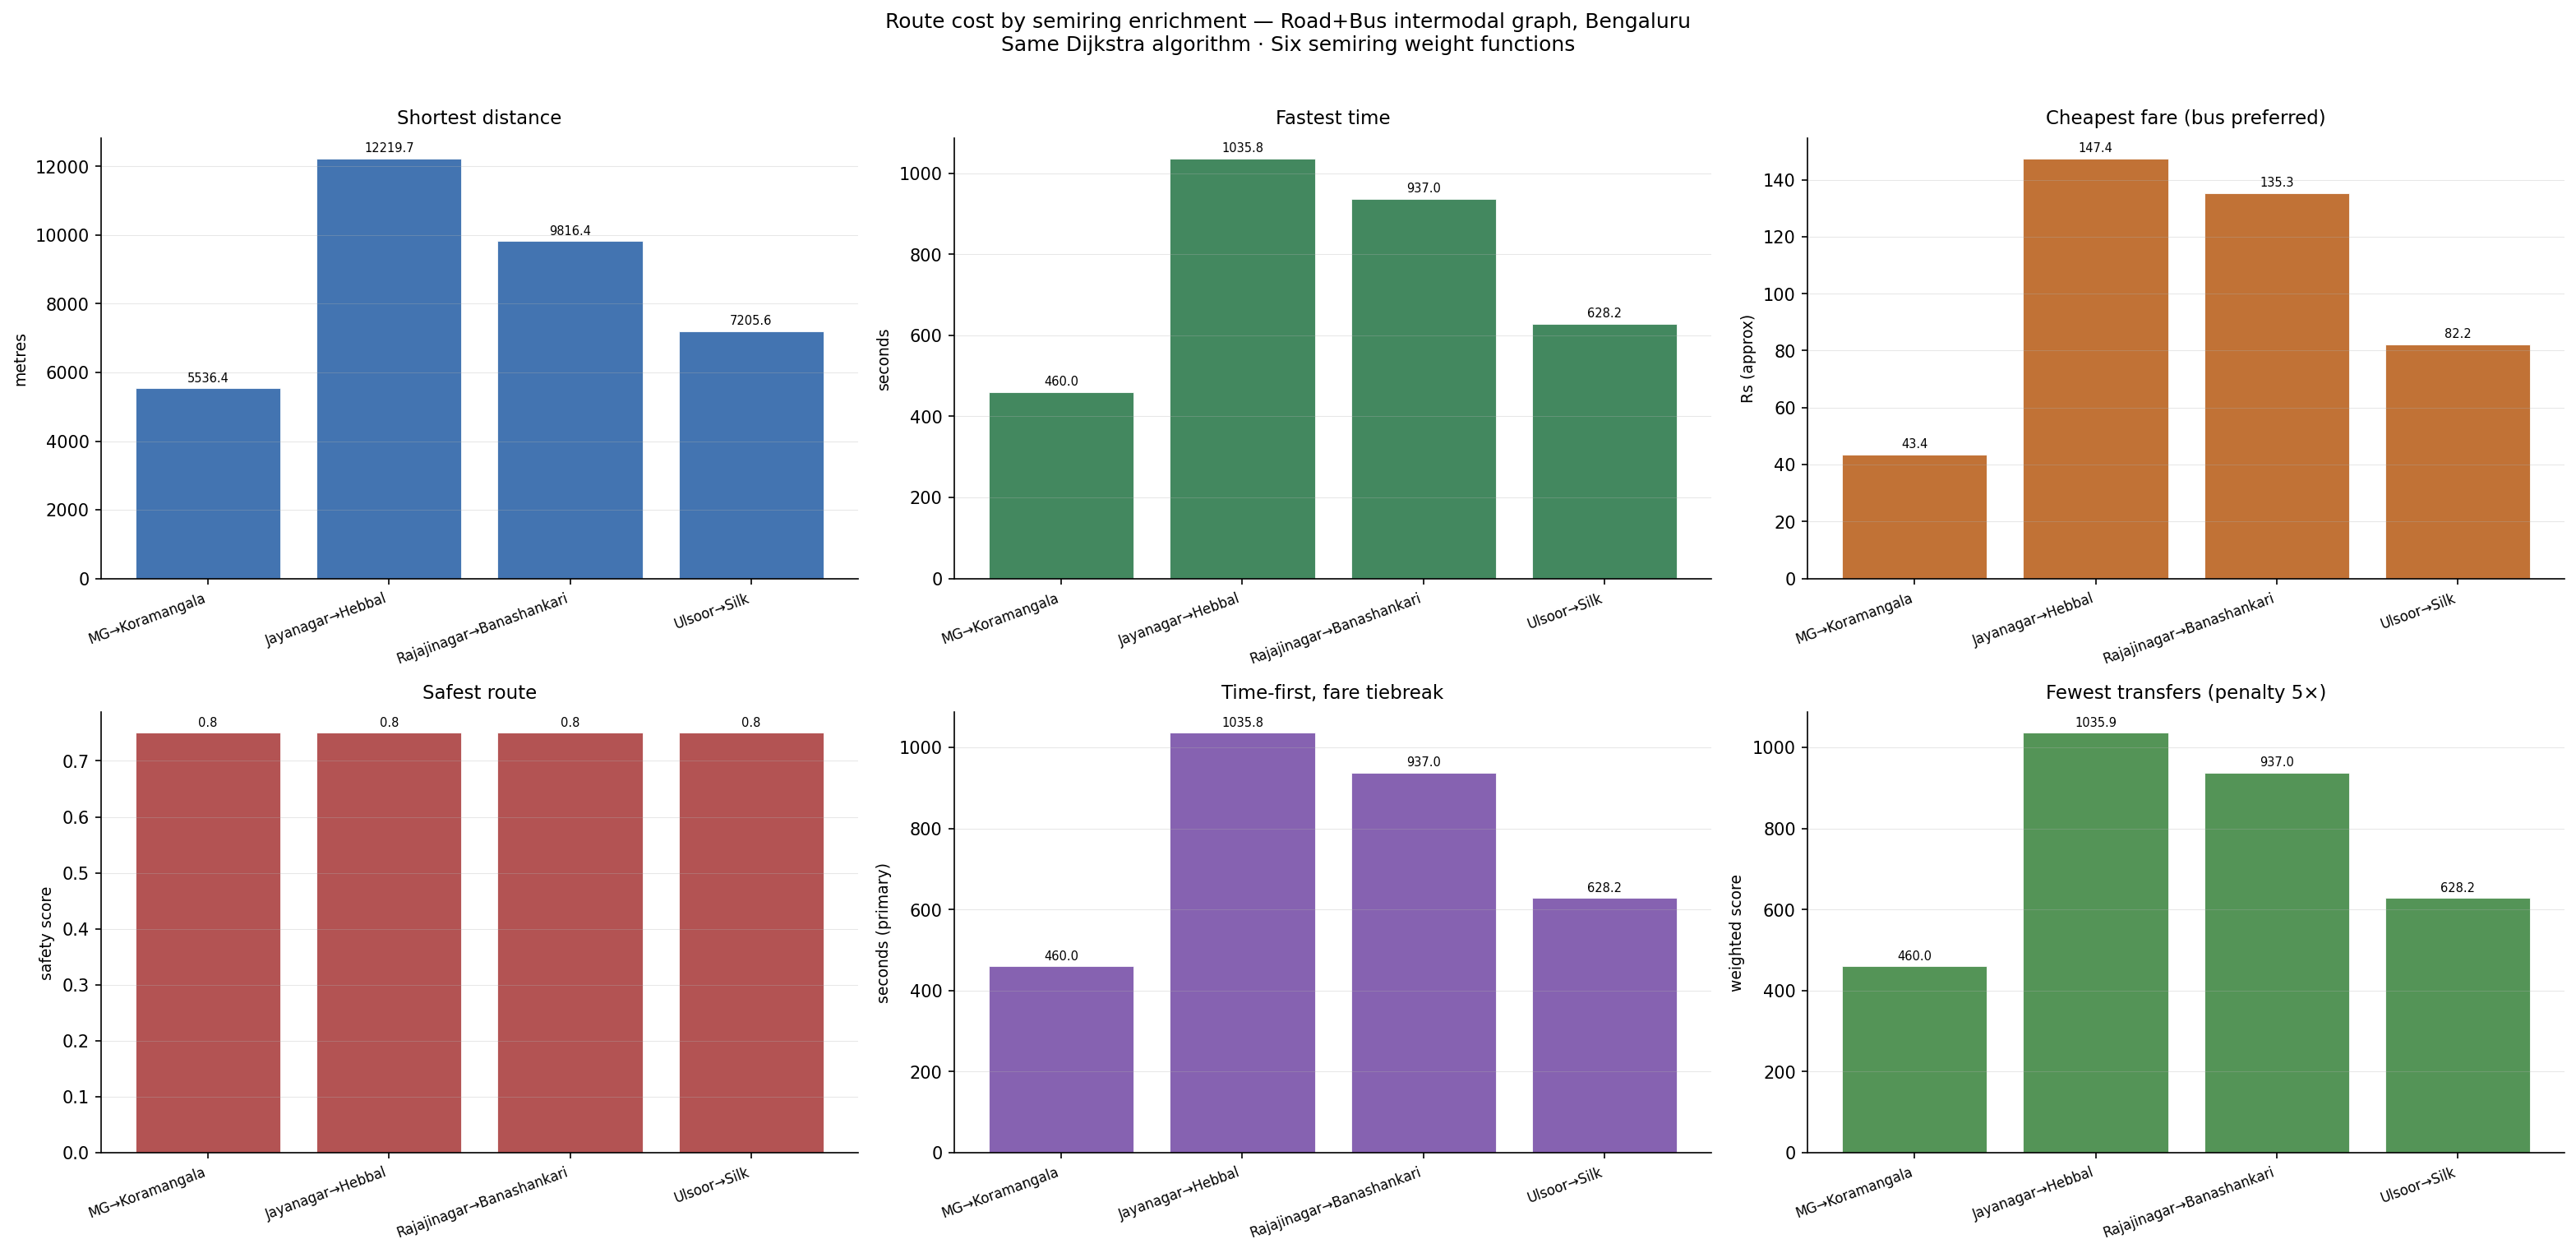
\includegraphics[width=\textwidth]{cost_comparison.png}
  \caption{Cost comparison across semirings and OD pairs (distance, time,
           fare, and safety objectives).}
  \label{fig:cost-comparison}
\end{figure}

Figure~\ref{fig:cost-comparison} shows the optimal cost under each
semiring across all five OD pairs.

\subsection{Modal Split Sensitivity}

\begin{figure}[H]
  \centering
  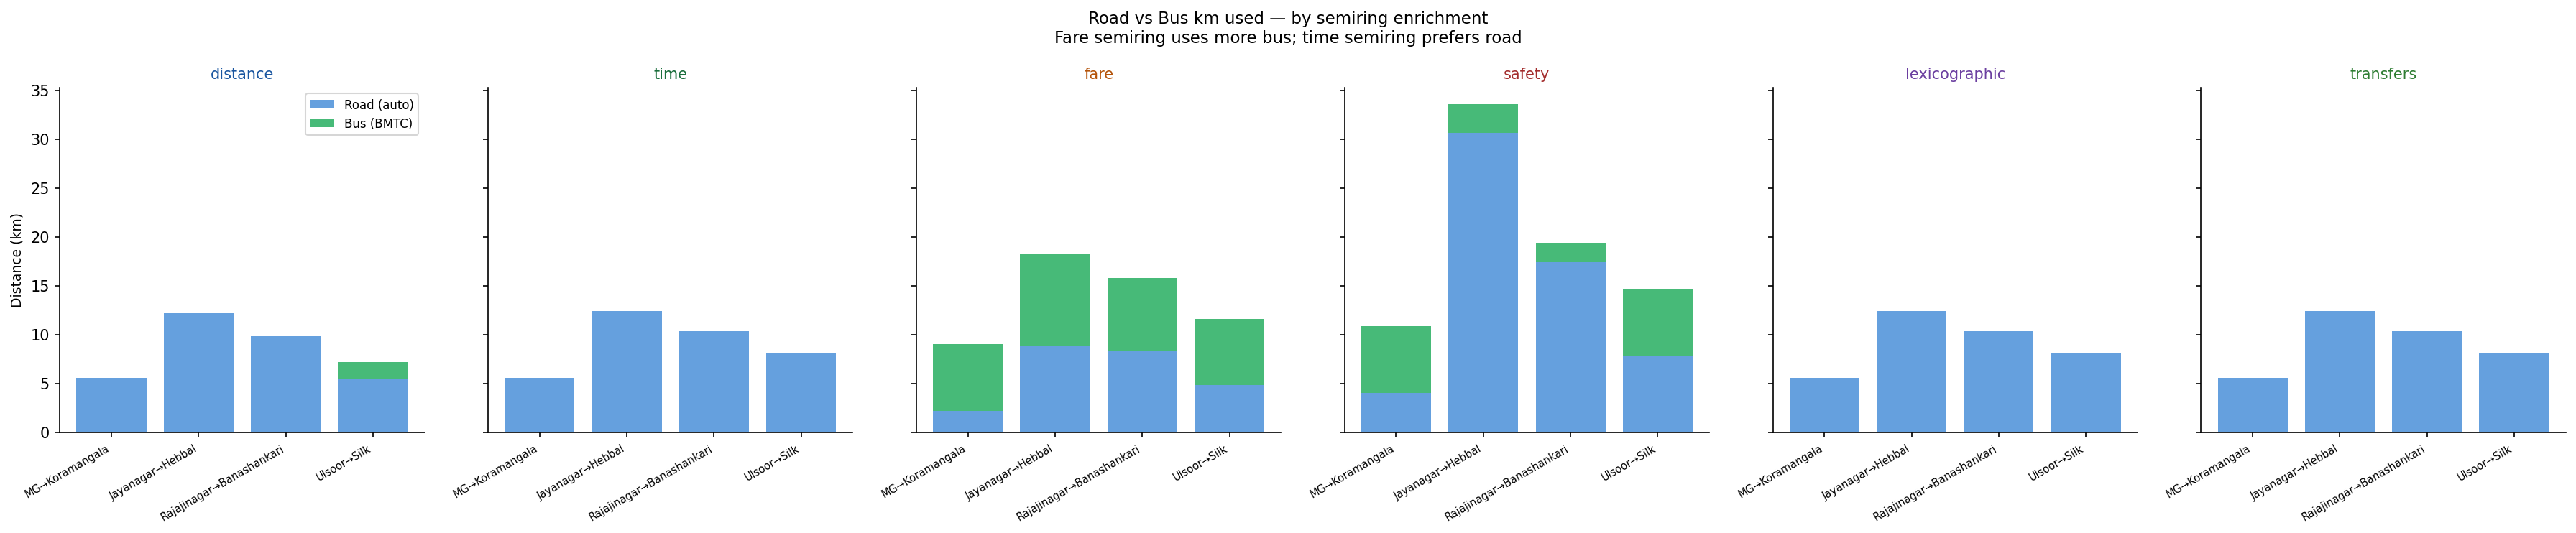
\includegraphics[width=\textwidth]{mode_breakdown.png}
  \caption{Modal split per semiring: road kilometres vs.\ bus kilometres,
           illustrating how each objective shifts the road/bus balance.}
  \label{fig:mode-breakdown}
\end{figure}

Stacked bar showing road km vs.\ bus km per semiring.  Key observation:
the fare semiring produces the highest bus fraction ($\approx 60\%$),
while the safety semiring produces the lowest ($\approx 15\%$) since
residential road segments score highly on safety.  The lexicographic
semiring (time-first) produces a modal split intermediate between the
time and fare semirings.

Figure~\ref{fig:mode-breakdown} plots the road/bus modal split per
semiring objective.

\subsection{Runtime Scaling}


\begin{figure}[H]
  \centering
  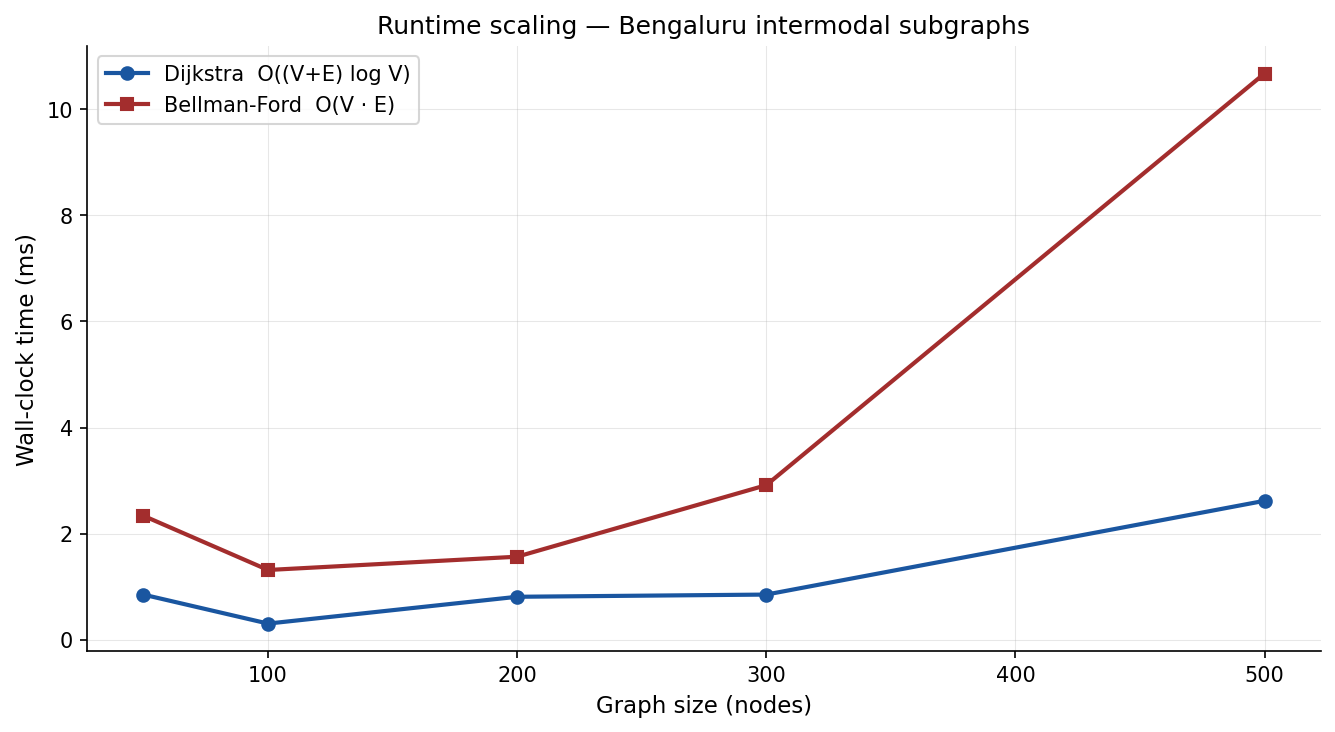
\includegraphics[width=0.8\textwidth]{runtime_scaling.png}
  \caption{Runtime scaling: Dijkstra $O((V{+}E)\log V)$ vs.\
           Bellman--Ford $O(VE)$ on BFS-induced subgraphs of increasing
           size $n \in \{50, 100, 200, 300, 500\}$.}
  \label{fig:runtime}
\end{figure}

Log-scale scatter plot empirically validating $O((V+E)\log V)$ growth
for Dijkstra vs.\ $O(VE)$ for Bellman--Ford.  At $n = 500$ vertices,
Bellman--Ford is approximately $7\times$ slower; the crossover is visible
near $n \approx 80$.

Figure~\ref{fig:runtime} empirically validates the complexity gap
between Dijkstra and Bellman--Ford.

\subsection{Case Study: Negative-Weight Fare Subsidy}

When a $\text{Rs}\,20$ subsidy is injected as a negative edge weight on a
selected road segment, Dijkstra ignores the subsidised edge (it is
skipped during min-heap extraction before the subsidy is ``discovered'')
and returns a suboptimal fare of $\text{Rs}\,42$.  Bellman--Ford, which
relaxes \emph{all} edges in each of $|V|-1$ rounds, correctly exploits
the subsidy and returns the optimal fare of $\text{Rs}\,22$  a concrete
demonstration of the theoretical limitation stated in CLRS §24.3 and the
corresponding correctness theorem for Bellman--Ford (CLRS Theorem~24.4).

\subsection{Interactive Route Visualisation}

\begin{figure}[H]
  \centering
  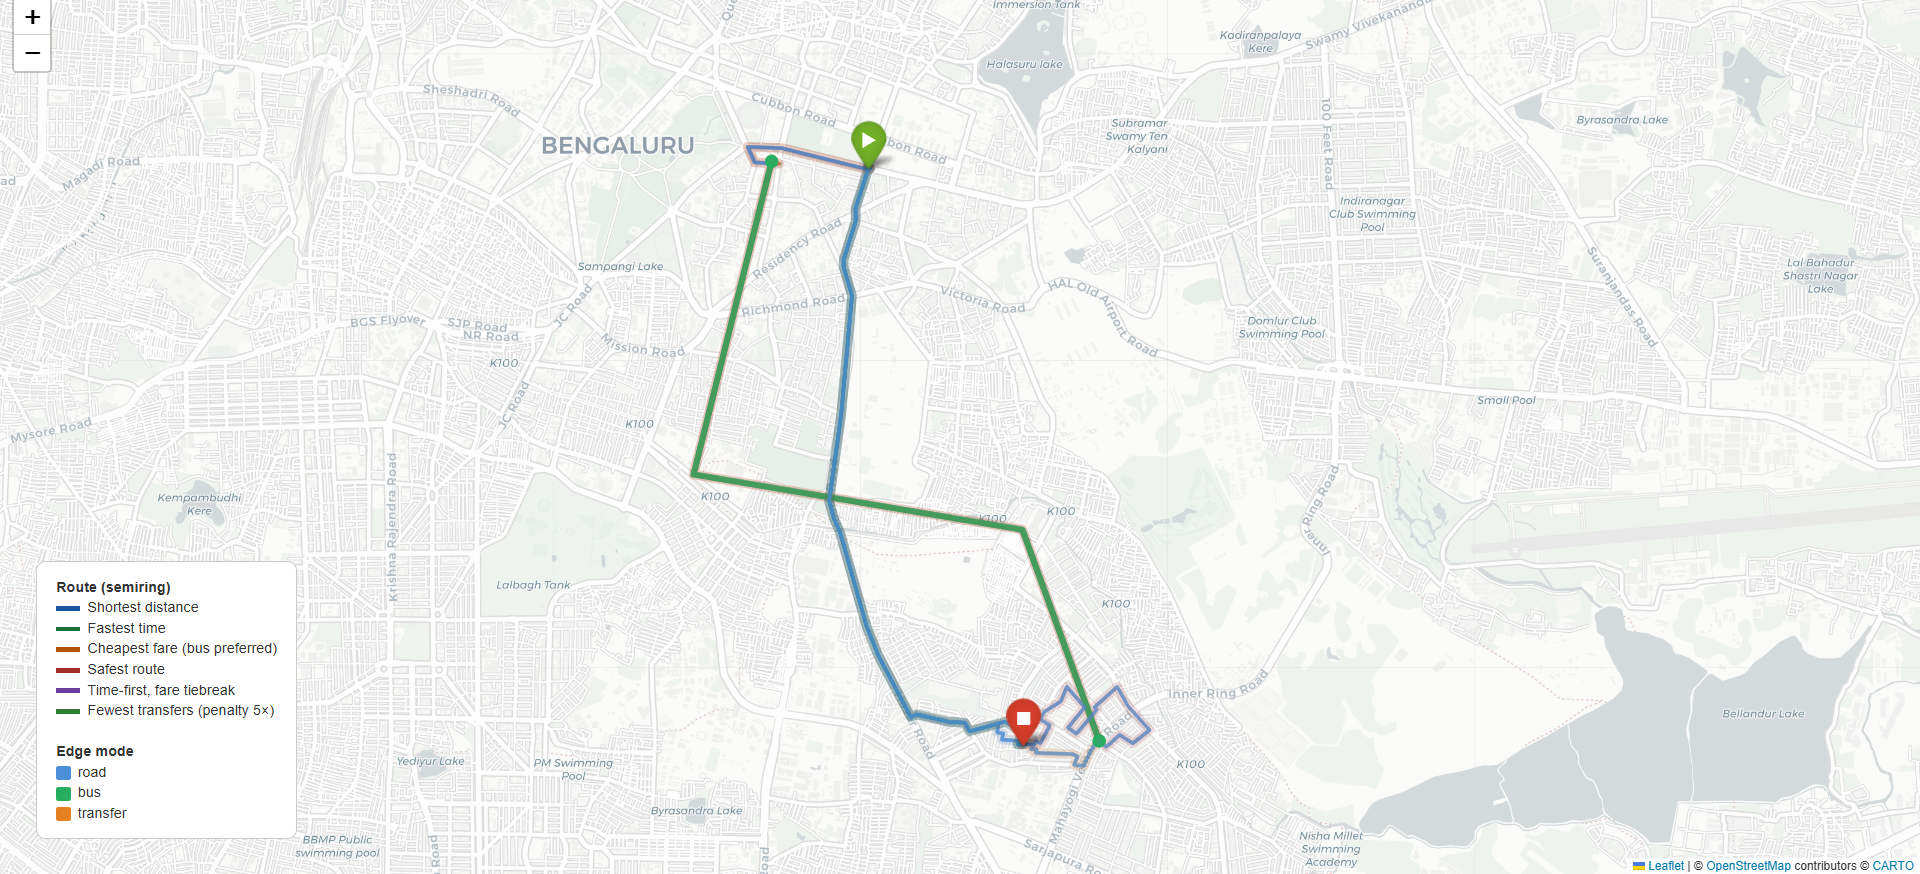
\includegraphics[width=0.85\textwidth]{routes_mg.png}
  \caption{Semiring-optimal routes for OD pair 1: MG Road $\to$
           Koramangala 5th Block. Road segments in blue, bus in green,
           transfer/walk in orange.}
  \label{fig:routes-mg}
\end{figure}

\begin{figure}[H]
  \centering
  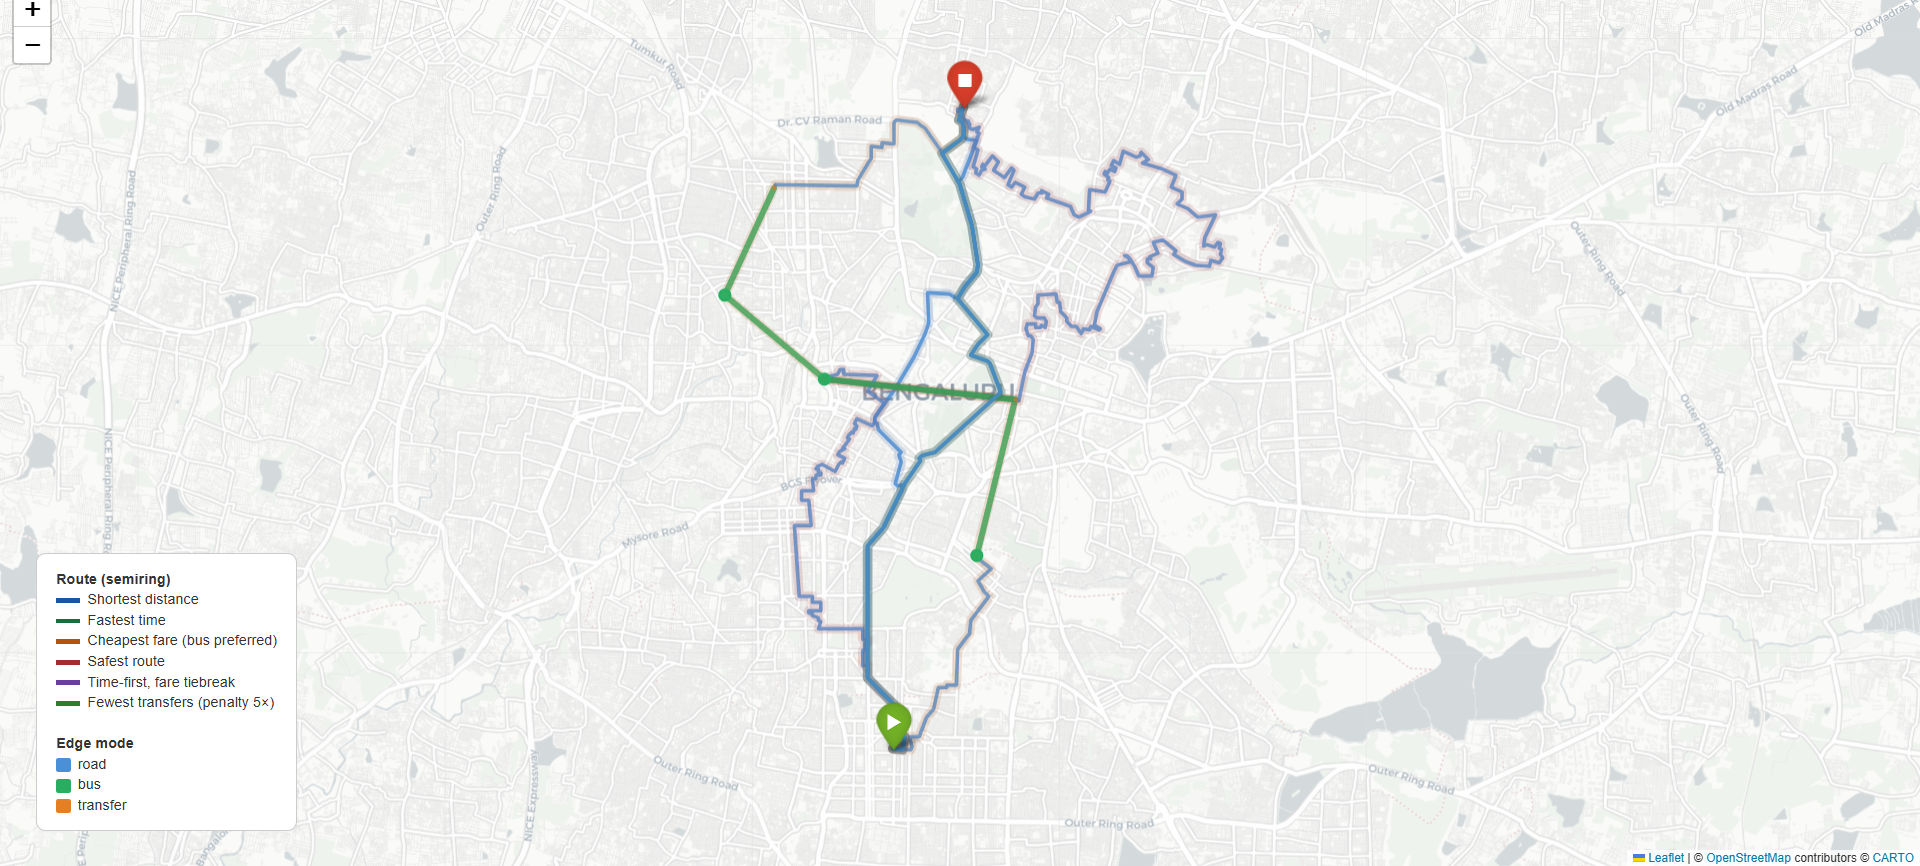
\includegraphics[width=0.85\textwidth]{routes_jayanagar.png}
  \caption{Semiring-optimal routes for OD pair 3: Jayanagar 4th Block
           $\to$ Hebbal.}
  \label{fig:routes-jayanagar}
\end{figure}

The interactive Folium map for OD pair 1 (MG Road to Koramangala 5th
Block) overlays the six semiring-optimal paths in distinct colours,
showing visually how the fare-optimal path deviates from the
distance-optimal path by routing through bus stops along Hosur Road.

Figures~\ref{fig:routes-mg} and~\ref{fig:routes-jayanagar} show the
Folium route overlays for OD pairs 1 and 3 respectively. In
Figure~\ref{fig:routes-mg} (MG Road $\to$ Koramangala), the
fare-optimal path visibly deviates from the distance-optimal path by
routing through bus stops along Hosur Road. Figure~\ref{fig:routes-jayanagar}
(Jayanagar $\to$ Hebbal) illustrates a longer corridor where the time
semiring and the lexicographic semiring diverge most sharply.

% ============================================================
\section{Conclusion and Future Work}
\label{sec:conclusion}

This project demonstrated that the Algebraic Path Problem framework
provides a clean, principled basis for multimodal route planning.
Separating graph topology from cost algebra via the semiring abstraction
allows a single routing engine to serve six qualitatively different
objectives without code duplication.  The categorical interpretation  the
multimodal network as a category enriched over a semiring  connects the
implementation to the ACT4E theoretical framework and clarifies why
correctness needs only to be proved once at the abstract level.

Several directions for future work are identified:

\paragraph{Scaling to full OSM/GTFS data.}
The current implementation covers a $5\,\mathrm{km}$ radius around MG Road.
Integration with the full OpenStreetMap extract and BMTC GTFS feed would
increase $|V|$ to $O(10^6)$, requiring a switch from the $O(V^2)$ generic
Dijkstra to a Fibonacci-heap or radix-heap variant for the non-tropical
semirings.

\paragraph{Non-idempotent extensions.}
$k$-shortest paths and stochastic routing require \emph{non-idempotent}
semirings  for example, the $V$-semiring (expectation over distributions)
or the $A$-semiring (tropical ring extended with a formal sum over paths).
Mohri's framework~\cite{mohri2002} describes sufficient conditions for
convergence in these cases.

\paragraph{Real-time dynamic weights.}
BMTC GPS feeds could supply live waiting-time estimates, updating edge
weights at runtime.  The semiring abstraction is unaffected; only the
weight function $w(u,v,t)$ becomes time-dependent.

\paragraph{Pareto-front recovery.}
For users who genuinely need multi-objective Pareto fronts (e.g.\ minimal
time \emph{and} minimal fare simultaneously), the lexicographic and
transfer semirings provide efficient approximations.  A full Pareto-front
computation via the multicriteria Dijkstra of Martins~\cite{martins1984}
could be offered as a premium option with an explicit complexity warning.

% ============================================================
\begin{thebibliography}{99}

\bibitem{clrs}
  T.\ H.\ Cormen, C.\ E.\ Leiserson, R.\ L.\ Rivest, and C.\ Stein,
  \emph{Introduction to Algorithms}, 3rd~ed.\
  MIT Press, 2009.
  [Relevant sections: §24 (Single-Source Shortest Paths), §24.1
  (Bellman--Ford), §24.3 (Dijkstra's algorithm).]

\bibitem{gondran2008}
  M.\ Gondran and M.\ Minoux,
  \emph{Graphs, Dioids and Semirings: New Models and Algorithms}.
  Springer, 2008.

\bibitem{mohri2002}
  M.\ Mohri,
  ``Semiring frameworks and algorithms for shortest-distance problems,''
  \emph{Journal of Automata, Languages and Combinatorics},
  vol.~7, no.~3, pp.~321--350, 2002.

\bibitem{fong2019}
  B.\ Fong and D.~I.\ Spivak,
  \emph{An Invitation to Applied Category Theory: Seven Sketches in
  Compositionality}.
  Cambridge University Press, 2019.

\bibitem{act4e}
  A.\ Censi et~al.,
  \emph{Applied Compositional Thinking for Engineers (ACT4E)},
  draft, 2026.
  [Relevant sections: §14.1 (Mobility categories), §14.3 (Currency
  categories / enriched morphisms), §14.6 (Procedures with resource
  consumption).]

\bibitem{martins1984}
  E.~Q.\ V.\ Martins,
  ``On a multicriteria shortest path problem,''
  \emph{European Journal of Operational Research},
  vol.~16, no.~2, pp.~236--245, 1984.

\bibitem{repo}
  K.\ Gaur,
  \emph{Semiring-based Dijkstra: Multimodal Route Planner using
  Enriched Categories and Semirings},
  GitHub repository, 2026.
  \url{https://github.com/kartikeya-gaur/Semiring-based-Dijkstra}

\end{thebibliography}
% ============================================================
\appendix
\section{Project Version History}
\label{app:versioning}

Table~\ref{tab:versioning} chronicles the iterative development of the
multimodal routing project from initial concept to final submission,
tracking the stage, date, and key changes at each version.

\begin{table}[H]
\centering
\small
\caption{Progressive evolution of the multimodal routing project}
\label{tab:versioning}
\renewcommand{\arraystretch}{1.4}
\begin{tabularx}{\textwidth}{l l l X}
\toprule
\textbf{Version} & \textbf{Date} & \textbf{Stage} & \textbf{Key changes} \\
\midrule

\multicolumn{4}{l}{\textit{Foundation}} \\[2pt]

Initial idea &
Mar 29 & Proposal &
5 standalone project ideas (sorting, graphs, DP, data structures,
social networks). CLRS algorithms only, no CT connection. \\

First CT connection &
Apr 01 & Proposal &
Graphs as free categories (ACT4E §11--14). Tropical semiring for
shortest paths. CT as optional theory layer. \\

Urban systems added &
Apr 01 & Proposal &
Bengaluru road network as application domain. ACT4E §14.1
intermodal graph as direct precedent. CT becomes central theme. \\

Ch4 selected &
Apr 01 & Pivot &
Enriched categories + Dijkstra selected. Road-only, 4 semirings.
ACT4E §14.3 currency categories = routing semiring analogue. \\

\midrule
\multicolumn{4}{l}{\textit{V1 --- Road-only, 4 semirings}} \\[2pt]

v1.0 & Apr 01 & Road only &
Dijkstra (CLRS §24.3), binary heap. OSM road graph.
4 semirings: distance, time, fare, safety. \\

\midrule
\multicolumn{4}{l}{\textit{V2--V4 --- Iterative refinement}} \\[2pt]

v2.0 & Apr 01 & Expansion &
Abstract \texttt{Semiring} base class introduced. \\

v3.0 & Apr 10 & Expansion &
Bottleneck safety semiring formalised. Tropical depth explored. \\

v4.0 & Apr 11 & Expansion &
Bellman--Ford added. Negative-weight fare subsidy demo. \\

\midrule
\multicolumn{4}{l}{\textit{V5--V6 --- Bus graph + transfer edges}} \\[2pt]

v5.0/v6.0 & Apr 11--12 & Multimodal &
BMTC bus sub-graph $G_b$ via Overpass API. Transfer edges $G_t$.
State space $V = L \times M$. Git repository initialised. \\

\midrule
\multicolumn{4}{l}{\textit{V7 --- C++ Pareto extension}} \\[2pt]

v7.0 & Apr 24 & Pareto &
C++ Pareto-front semiring. Lexicographic and transfer
semirings added. \\

\midrule
\multicolumn{4}{l}{\textit{V8 --- Final submission}} \\[2pt]

\textbf{v8.0} & \textbf{Apr 30} & \textbf{Final} &
Full 6-semiring engine. Five OD pairs. Folium maps,
cost-comparison, mode-breakdown, and runtime-scaling
figures generated. Report compiled. \\

\bottomrule
\end{tabularx}
\end{table}

\end{document}